% Intended LaTeX compiler: pdflatex
\documentclass[10pt,a4paper,UTF8]{article}
\usepackage{zclorg}
\author{emacsun}
\date{}
\title{曲线拟合之matlab实现}
\hypersetup{
 pdfauthor={emacsun},
 pdftitle={曲线拟合之matlab实现},
 pdfkeywords={},
 pdfsubject={},
 pdfcreator={Emacs 25.0.50.1 (Org mode 9.0.6)},
 pdflang={English}}
\begin{document}

\maketitle
\tableofcontents
\titlepic{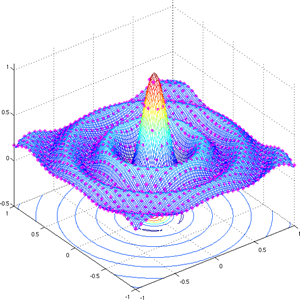
\includegraphics[scale=0.25]{../../img/sinc.PNG}}

\section{回忆}
\label{sec:org5ef0dd1}


在
\begin{enumerate}
\item \href{./PRMLch1dot1-polynomial-curve.org}{多项式拟合到模式识别的相关概念}
\item \href{./PRMLch1dot1-polynomial-curve-appendix.org}{曲线拟合过程中的欠定过定问题}
\item \href{./PRMLch1dot1-polynomial-curve-probability-revist.org}{曲线拟合之概率回访}
\end{enumerate}

中我们介绍了多项式曲线拟合问题并从多方面对其进行了分析,顺便引入了机器学习领域的一些关键术语。今天我们针对多项式曲线拟合问题做一些matlab试验。
\subsection{数学模型}
\label{sec:org4539d06}


目标模型:
\begin{equation}
\label{eq:2}
y(x, \mathbf{w}) = w_{0} + w_{1}x + \ldots + w_{M}x^{M} = \sum_{j=0}^{M}w_{j}x^{j}
\end{equation}
均方误差函数:
\begin{equation}
\label{eq:3}
E( \mathbf{w}) = \frac{1}{2} \sum_{n=1}^{N}\{y(x_{n}, \mathbf{w}) - t_{n}\}^{2}
\end{equation}
针对目标模型和均方误差函数的解\(\mathbf{w} = \{w_{j}\}\)是一般线性方程:
\begin{equation}
\label{eq:4}
\sum_{j=0}^{M}A_{ij}w_{j} = T_{i}, i = 0,\ldots ,M
\end{equation}
的解。其中\(A_{ij} = \sum_{n=1}^{N}(x_{n})^{i+j}\),\(T_{i} = \sum_{n=1}^{N}(x_{n})^{i}t_{n}\) 关于这个结论的证明过程详见 \href{./PRMLch1dot1-polynomial-curve-appendix.org}{曲线拟合过程中的欠定过定问题} 。

式 (\ref{eq:4}) 可以写成矩阵的形式,如下:

\begin{equation}
\label{eq:1}
\begin{bmatrix}
A_{00} & \ldots & A_{0M}\\
\vdots & \ddots & \vdots \\
A_{M0} & \ldots & A_{MM}
\end{bmatrix}
\begin{bmatrix}
w_{0} \\ \vdots \\ w_{M}
\end{bmatrix}
=
\begin{bmatrix}
T_{0} \\ \vdots \\ T_{M}
\end{bmatrix}
\end{equation}

\subsection{正则化过程}
\label{sec:orgd072833}


针对误差函数 (\ref{eq:3})出现高阶模型的过拟合问题,对(\ref{eq:3}) 添加一个正则项会产生比较好的效果,如:
\begin{equation}
\label{eq:5}
E( \mathbf{w}) = \frac{1}{2} \sum_{n=1}^{N}\{y(x_{n}, \mathbf{w}) - t_{n}\}^{2} + \frac{\lambda}{2} \| \mathbf{w} \|^{2}
\end{equation}
其中\(\| \mathbf{w} \|^{2} = w_{0}^{2} + \ldots w_{M}^{2}\) ,稍后我们会看到这种正则化方法对于克服过拟合问题非常有效。针对式 (\ref{eq:5}) 和式 (\ref{eq:2}) 的解可以写成如下形式的解:
\begin{equation}
\label{eq:7}
\sum_{j=0}^{M}(A_{ij} + \lambda \delta_{ij})w_{j} = T_{i}, i = 0,\ldots ,M
\end{equation}
其中:
\begin{equation}
\label{eq:8}
\delta_{ij} =
\begin{cases}
1 & i = j \\
0 & i\neq j
\end{cases}
\end{equation}
矩阵形式就是:
\begin{equation}
\label{eq:6}
\begin{bmatrix}
A_{00} - \lambda  & \ldots & A_{0M}\\
\vdots & \ddots & \vdots \\
A_{M0} & \ldots & A_{MM} - \lambda
\end{bmatrix}
\begin{bmatrix}
w_{0} \\ \vdots \\ w_{M}
\end{bmatrix}
=
\begin{bmatrix}
T_{0} \\ \vdots \\ T_{M}
\end{bmatrix}
\end{equation}
式\textasciitilde{}(\ref{eq:6})和式 (\ref{eq:1}) 的区别在于,矩阵\(A\)的对角线上有一个\(\lambda\)的修正(或者叫做惩罚)。这样做的好处是求得的系数\(\mathbf{w}\)不会太大。
\section{matlab实现}
\label{sec:orgdcba2d5}

\subsection{画出\(y = \sin (2\pi x)\)}
\label{sec:orge19ee2a}
  \textit{[2017-05-21 Sun 15:55]}
首先我们画出\(y = \sin (2\pi x)\),这个函数的图像:
\lstset{language=matlab,label= ,caption= ,captionpos=b,firstnumber=1,numbers=left}
\begin{lstlisting}
x = 0:0.01:1;%x
y = sin(2* pi * x);
figure
plot(x,y,'-r','linewidth',2),hold on;
\end{lstlisting}
结果如图\ref{fig:org46d6919} 所示:
\begin{figure}[htbp]
\centering
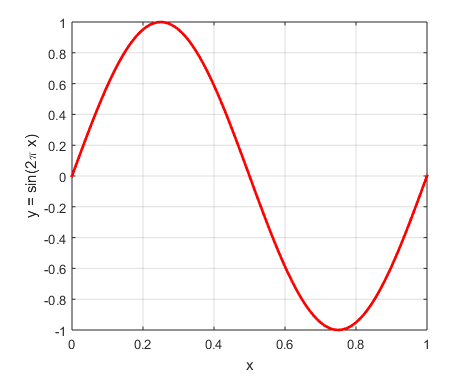
\includegraphics[width=0.6\textwidth]{../../img/computer_prml/20170521figure1.png}
\caption{\label{fig:org46d6919}
\(y = \sin(2*\pi x)\)}
\end{figure}
\subsection{训练集合}
\label{sec:org6c992ad}
   \textit{[2017-05-21 Sun 15:55]}
然后给出一个训练集合,并画出这个集合的图像:
\lstset{language=matlab,label= ,caption= ,captionpos=b,firstnumber=1,numbers=left}
\begin{lstlisting}
numTraining = 100;
xTraining = rand(1,numTraining);
noiseVariance = 0.5;
noise = noiseVariance *randn(1,numTraining);
yTraining = sin(2*pi*xTraining) + noise;
plot(xTraining,yTraining,'b+','linewidth',2),hold on;
\end{lstlisting}
和\(y = \sin(2\pi x)\)画在一张图上,如图所示:
\begin{figure}[htbp]
\centering
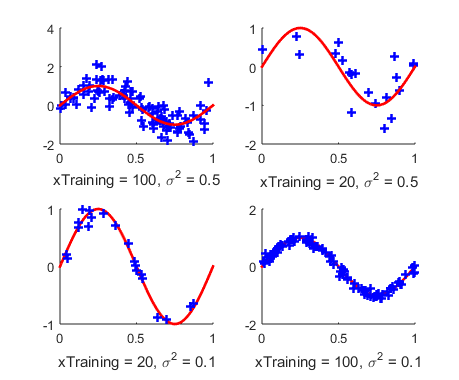
\includegraphics[width=0.6\textwidth]{../../img/computer_prml/20170521figure2.png}
\caption{\label{fig:org7b5b9d5}
训练集合}
\end{figure}

注意这里有两个地方可以做调整:1. 训练结合的数量 \texttt{numTraining} ;2. 噪声的方差 \texttt{noiseVariance} .不同的训练集合大小和方差会影响最终的训练效果。当然总体结论是:训练集合越大,方差越小,训练效果越好。
\subsection{曲线拟合}
\label{sec:org9e26143}


曲线拟合的过程就是计算\(\mathbf{w}\)的过程,首先我们观察式\textasciitilde{}(\ref{eq:4}) 的结果。我们把计算\(Ax=B\)的过程分为三步:
\begin{enumerate}
\item \texttt{getA}
\item \texttt{getB}
\item \texttt{A\textbackslash{}B}
\end{enumerate}
这三步的代码:
\lstset{language=matlab,label= ,caption= ,captionpos=b,firstnumber=1,numbers=left}
\begin{lstlisting}
%%find the A and B for Ax = B
A = getA(xTraining,modelOrder);
B = getB(xTraining,yTraining,modelOrder);
w = A\B';
for i = 1:length(x)
yEstimation(i) = x(i).^(0:modelOrder ) * w  ;
end
\end{lstlisting}

先是 \texttt{getA}
\lstset{language=matlab,label= ,caption= ,captionpos=b,firstnumber=1,numbers=left}
\begin{lstlisting}
function A = getA(xTraining,modelOrder)
    for i = 1:modelOrder + 1
        for j = 1:modelOrder + 1
            A(i,j) = sum(xTraining.^(i+j - 2));
        end
    end
end
\end{lstlisting}
然后 \texttt{getB}
\lstset{language=matlab,label= ,caption= ,captionpos=b,firstnumber=1,numbers=left}
\begin{lstlisting}
function B = getB(xTraining,yTraining,modelOrder)
   for i = 1:modelOrder + 1
       B(i) = sum(yTraining .* xTraining.^(i-1));
   end
end
\end{lstlisting}

我们给出 训练集合大小为20,模型阶数为9的训练结果:
\begin{figure}[htbp]
\centering
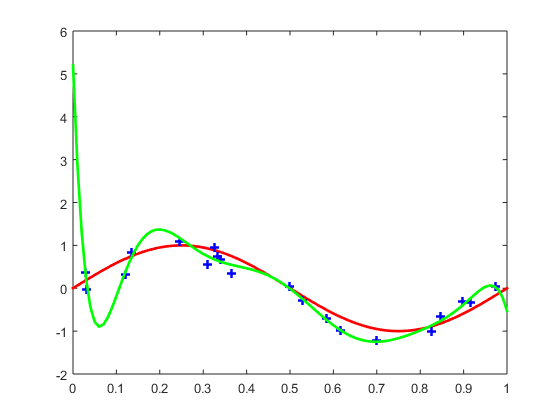
\includegraphics[width=0.6\textwidth]{../../img/computer_prml/20170521figure3.png}
\caption{\label{fig:org70e93f0}
训练集合大小为20,模型阶数为9的训练结果}
\end{figure}

图中绿色曲线就是训练结果,可以看出来这个结果显然是过拟合了。我们给出来训练集合大小为20,模型结束为5的训练结果:
\begin{figure}[htbp]
\centering
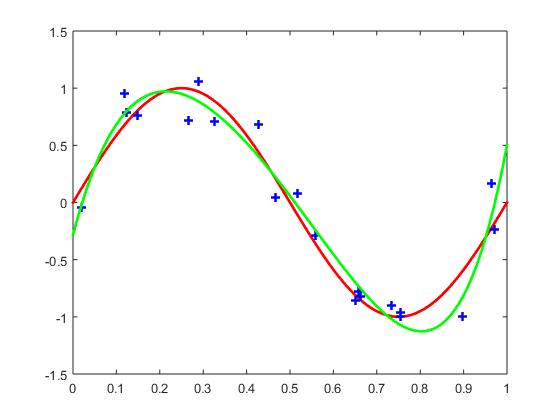
\includegraphics[width=0.6\textwidth]{../../img/computer_prml/20170521figure4.png}
\caption{\label{fig:org85b7169}
训练集合大小为20,模型阶数为5的训练结果}
\end{figure}
\subsection{正则化}
\label{sec:org8e48453}


按照式 (\ref{eq:7}) 所给结果,设置\(\lambda = 0.001\),设置模型阶数为9,训练集合大小为20,训练结果:
\begin{figure}[htbp]
\centering
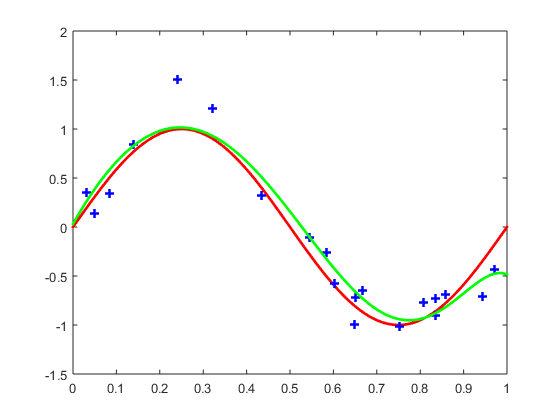
\includegraphics[width=0.6\textwidth]{../../img/computer_prml/20170521figure5.png}
\caption{\label{fig:org056b7ef}
训练集合大小为20,模型阶数为9的训练结果,\(\lambda = 0.001\)}
\end{figure}

从图\ref{fig:org056b7ef} 和 \ref{fig:org70e93f0} 可以看到,正则化有效的遏制了拟合结果波动过大的情况。

\section{下载完整的代码}
\label{sec:orge86e31b}


\href{curve\_fitting.m}{下载完整的代码}。
\end{document}